% Created 2025-01-14 Tue 19:10
% Intended LaTeX compiler: pdflatex
\documentclass[presentation]{beamer}
\usepackage[utf8]{inputenc}
\usepackage[T1]{fontenc}
\usepackage{graphicx}
\usepackage{amsmath, amssymb}
\usepackage{hyperref}
\setbeamertemplate{navigation symbols}{}
\usepackage[utf8]{inputenc}
\usepackage[T1]{fontenc}
\usepackage{graphicx}
\usepackage{longtable}
\usepackage{wrapfig}
\usepackage{rotating}
\usepackage[normalem]{ulem}
\usepackage{amsmath}
\usepackage{amssymb}
\usepackage{capt-of}
\usepackage{hyperref}
\nocite{*}
\usepackage[T1]{fontenc}
\usepackage[utf8]{inputenc}
\usepackage[spanish]{babel}
\usepackage[backend=biber, style=apa]{biblatex}
\addbibresource{/home/iccd332-josune/expo/ExposicionArqui/bibliography.bib}
\author{Lenin G. Falconí, Richard Dawkins, Jean LeCunn}
\date{}
\title{S9-Memoria-del-Sistema}
\hypersetup{
 pdfauthor={Lenin G. Falconí, Richard Dawkins, Jean LeCunn},
 pdftitle={S9-Memoria-del-Sistema},
 pdfkeywords={},
 pdfsubject={},
 pdfcreator={Emacs 27.1 (Org mode 9.3)}, 
 pdflang={Spanish}}
\begin{document}

\maketitle
\tableofcontents



\section{Indicaciones}
\label{sec:orgae5bc0c}
\subsection{Indicaciones}
\label{sec:org23ada82}
\subsection{Diseño de las Diapositivas}
\label{sec:org60704b1}
\begin{itemize}
\item Para diseñar sus diapositivas puede consultar cualquiera de las
presentaciones .ORG desarrolladas por el profesor así como al
archivo \href{https://github.com/LeninGF/EPN-Lectures/blob/main/iccd332ArqComp-2024-B/Tutoriales/Beamer-Emacs/tutorialBeamer.org}{tutorialBeamer.org} en el repositorio de \href{https://github.com/LeninGF/EPN-Lectures/blob/main/iccd332ArqComp-2024-B/Tutoriales/Beamer-Emacs/tutorialBeamer.org}{GitHub} de la clase.
\item Recuerde que los archivos .ORG son archivos de texto así que los
puede copiar y sustituir por su texto propio.
\end{itemize}
\subsection{Sobre este Documento}
\label{sec:orgc4bfac1}
\begin{itemize}
\item Este documento tiene la propuesta de temas a tratar y desarrollar
por los estudiantes.
\item Se ha de utilizar como base la bibliografía recomendada, pero puede
consultar bibliografía adicional.
\end{itemize}
\section{Memoria Cache (E2, 11, 162)}
\label{sec:org5c2d986}
\subsection{Principios Básicos de las Memorias Caché (E2,11,163)(E2,7,133)}
\label{sec:orgf150a23}
\textbf{\textbf{\textbf{¿Para que sirve?}}} 


El objetivo principal de la memoria caché es mejorar la velocidad de acceso a los datos almacenados, combinando el acceso rápido a datos de una memoria más cara y de alta velocidad (memoria caché) con el almacenamiento más lento pero de mayor capacidad de la memoria principal.


\textbf{\textbf{\textbf{Funcionamiento}}}


\begin{itemize}
\item La CPU transfiere palabras o bloques entre la caché y la memoria principal. La caché actúa como intermediaria rápida entre la CPU y la memoria principal, almacenando temporalmente datos que la CPU necesita frecuentemente.
\end{itemize}


\subsection{Principios Básicos de las Memorias Caché (E2,11,163)(E2,7,133)}
\label{sec:org73bf613}

\begin{itemize}
\item En el modelo simple de caché (como muestra la Figura 5.1a), la CPU realiza transferencias rápidas a la caché y transferencias más lentas a la memoria principal.
\end{itemize}

\begin{center}
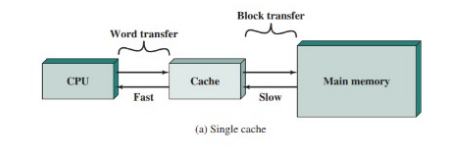
\includegraphics[width=.9\linewidth]{./Imagenes/captura1.png}
\end{center}

\subsection{Principios Básicos de las Memorias Caché (E2,11,163)(E2,7,133)}
\label{sec:org644d7aa}

Niveles de Caché: Se organizan en varios niveles (L1, L2, L3). A medida que se avanza en los niveles, la velocidad disminuye, pero la capacidad aumenta.

\begin{itemize}
\item Caché de Nivel 1 (L1): La más rápida y de menor capacidad.
\item Caché de Nivel 2 (L2): Un poco más lenta, pero con mayor capacidad.
\item Caché de Nivel 3 (L3): Menos rápida que L1 y L2, pero aún más rápida que la memoria principal.
\end{itemize}


\begin{enumerate}
\item Elementos de Diseño de la memoria Caché
\label{sec:org64e11e4}
\item Introducción a la Caché
\label{sec:org6a5b5a5}
\begin{itemize}
\item "La memoria caché mejora la velocidad de acceso
al reducir la distancia entre el procesador y la memoria principal."
\item "Los fallos de caché generan tráfico en el bus del sistema."
\end{itemize}
\begin{center}
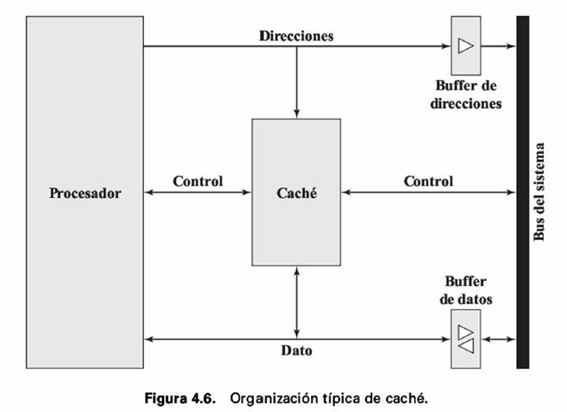
\includegraphics[width=.9\linewidth]{./Imagenes/fig4.6.png}
\end{center}
\item Parámetros de Diseño de la Caché
\label{sec:org6c816c6}
\begin{itemize}
\item "La función de correspondencia, el tamaño de línea y el algoritmo de sustitución
son clave para el diseño de una caché eficiente."
\item "La jerarquía de cachés puede mejorar el rendimiento en aplicaciones bien optimizadas."
\begin{center}
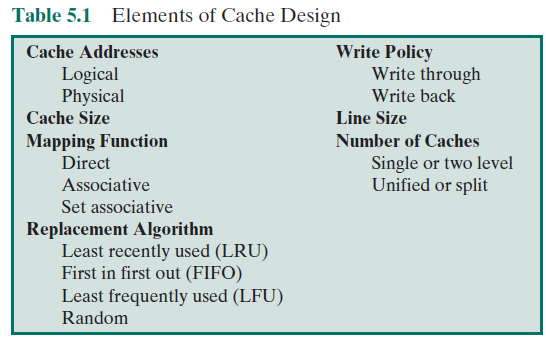
\includegraphics[width=.9\linewidth]{./Imagenes/tabla5.1.png}
\end{center}
\end{itemize}


\item Tamaño Caché
\label{sec:org7a88896}
\begin{itemize}
\item "El tamaño de la caché impacta directamente en su velocidad y costo."
\item "No existe un tamaño 'óptimo' único, ya que depende de la naturaleza de las tareas."
\begin{center}
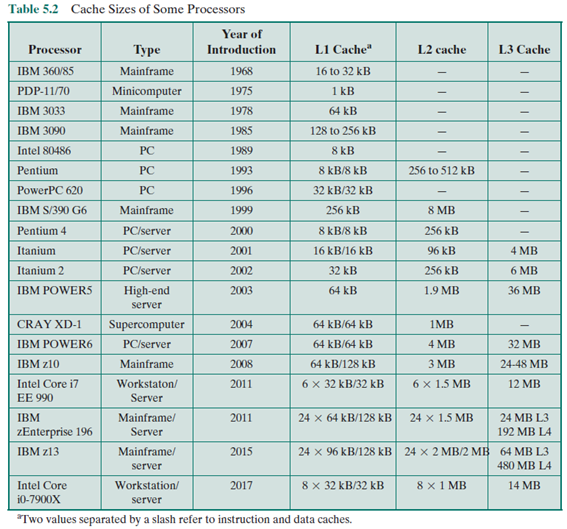
\includegraphics[width=.9\linewidth]{./Imagenes/tabla5.2.png}
\end{center}
\end{itemize}

\item Tipos de caché
\label{sec:orgd9bb906}
\begin{itemize}
\item "La caché lógica utiliza direcciones virtuales; la física, direcciones físicas."
\item "La caché lógica puede ser más rápida pero requiere mayor gestión en cambios de contexto."
\begin{center}
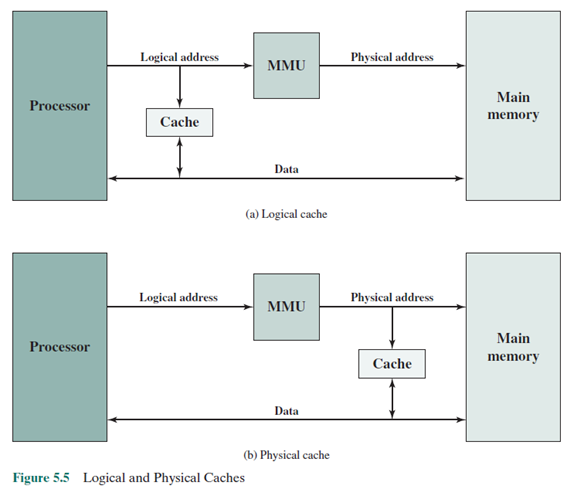
\includegraphics[width=.9\linewidth]{./Imagenes/fig5.png}
\end{center}
\end{itemize}
\end{enumerate}




\subsection{Función de Correspondencia (E2,11,170)(E2,7,137)}
\label{sec:orge603259}
\begin{itemize}
\item Se recomienda la tabla 5.3 página 170 de la 10ma edición
\end{itemize}
\subsection{Algoritmo de Sustitución (E2,7,148)}
\label{sec:orgec129b6}
\subsection{Política de escritura}
\label{sec:orgedec68d}
\subsection{Tamaño de Línea}
\label{sec:orgd75b599}
\subsection{Número de Cachés (E2, 7, 150)}
\label{sec:org57d8a1b}
\begin{itemize}
\item \autocite{stallings2006} página 172
\item \autocite{stallings2022computer} página 201 Capítulo 6
\end{itemize}

\section{Referencias}
\label{sec:org2c9c595}
\subsection{Bibliografía}
\label{sec:org17f32cf}
\printbibliography
\end{document}
